%Checklist: Spellcheck, style commands

\providecommand*\ExtraDocOpts{}
\documentclass[9pt,\ExtraDocOpts]{beamer}

%Make locally deterministic
\pdfinfo{ /Creator ()  /Producer () /ModDate ()  /CreationDate () }
\pdftrailerid{} %Remove ID
\pdfsuppressptexinfo15 %Suppress PTEX.Fullbanner and info of imported PDFs

\usepackage{etex} % Weird problem on dimensions
%\usetheme{spensiones}
%\mode<presentation> { \setbeamercovered{transparent} }
%\usepackage{stata}
\usepackage{tikz, tabularx, ulem}
%\usepackage{fancyvrb}
\usetikzlibrary{arrows, fit,positioning}
\usepackage{booktabs}

\title[{\tt parallel}]{Just tired of endless loops! \\ \textit{\footnotesize or} {\normalsize {\tt parallel}: Stata module for parallel computing}}

\author[Vega Yon, Quistorff]{George G. Vega Yon\inst{1} \and Brian Quistorff\inst{2}}
\institute[USC and MSR]{\inst{1}University of Southern California\\ vegayon@usc.edu\and \inst{2}Microsoft AI and Research\\Brian.Quistorff@microsoft.com}
\def\unix1{Intel Xeon X470 (hexadeca-core)}
\def\windows1{Intel i3 2120 (dual-core)}
\date{Stata Conference Baltimore\\July 27--28, 2017}
\begin{document}

\frame{
\maketitle
{\scriptsize
Thanks to Stata users worldwide for their valuable contributions. The usual disclaimers applies.}
}

\frame{
\frametitle{Agenda}
\tableofcontents
}

\section{Motivation}

\begin{frame} % [allowframebreaks=.8]
\frametitle{Motivation}
\begin{itemize}
\item Both computation power and size of data are ever increasing
\item Often our work is easily broken down into independent chunks \pause{}
\item Implementing parallel computing even for these ``embarrassingly parallel'' problems, however, is not easy.\pause{}
\item StataMP exists, but only parallelizes a limited set of internal commands, not user commands.\pause{}
\item {\tt parallel} aims to make this more convenient.\pause{}
\end{itemize}
\end{frame}

\section{What is it and how does it work}

\frame{\tableofcontents[currentsection]}

\begin{frame} % [allowframebreaks=.8]
\frametitle{What is it and how does it work}
\framesubtitle{What is it?}

\begin{itemize}
\item Inspired by the R package ``snow'' (several other examples exists: HTCondor, Matlab's Parallel Toolbox, etc.)\pause{}
\item Launches child batch-mode Stata processes across multiple processors (e.g.\ simultaneous multi-threading, multiple cores, sockets, cluster nodes).\pause{}
%\item By starting determined number of clusters (stata instances) this module was design to repeat a task simultaneously over the clusters.\pause{}
\item Depending on the task, can reach near linear speedups proportional to the number of processors.\pause{}
\begin{itemize}
\item Thus having a quad-core computer can lead to a 400\% speedup.
\end{itemize}
\end{itemize}

\end{frame}



\begin{frame}
\frametitle{Simple usage}

\begin{columns}
\begin{column}{.5\textwidth}
{\color{gray}
{\tt Serial: }
\rule{\linewidth}{4pt}}
\begin{itemize}
\item gen v2 = v*v
\item do byobs\_calc.do
\item bs, reps(5000): reg price foreign rep\pause{}
\end{itemize}
\end{column}%
\hfill%
\begin{column}{.5\textwidth}
{\color{gray}
{\tt Parallel:}
\rule{\linewidth}{4pt}}
\begin{itemize}
\item parallel: gen v2 = v*v
\item parallel bs, reps(5000): reg price foreign rep
\item parallel do byobs\_calc.do
\end{itemize}
\end{column}%
\end{columns}
\end{frame}


\begin{frame}[b]
\frametitle{What is it and how does it work}
\framesubtitle{How does it work?}
\begin{figure}
\centering
\scalebox{.7}{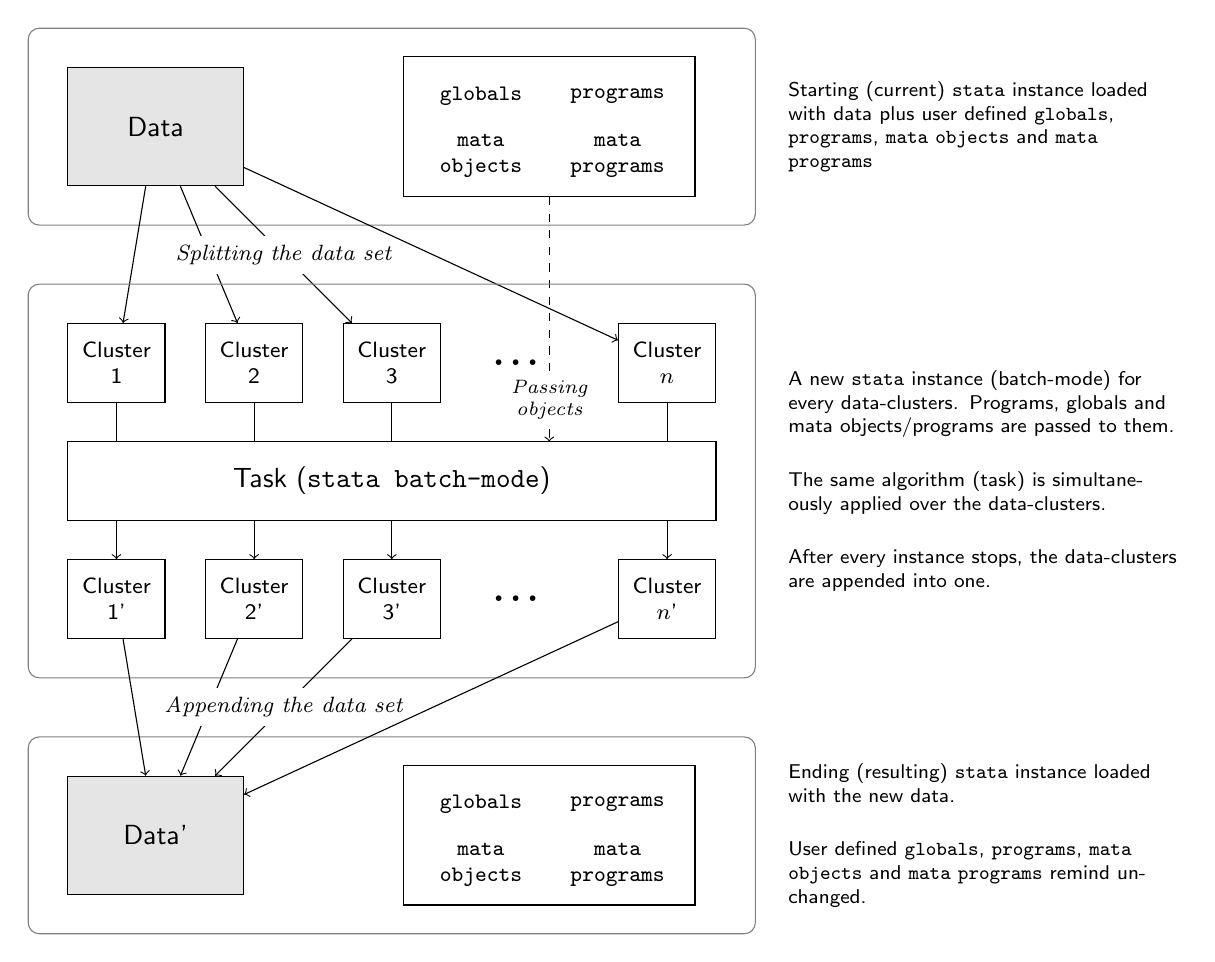
\begin{tikzpicture}[
	every node/.style={node distance=.5cm and .5cm, font=\sffamily}, 
	datablock/.style={rectangle, draw, fill=black!10, text width=2cm, minimum height=1.5cm, text badly centered},
	cluster/.style={rectangle, draw,text width=1cm, text badly centered, minimum height=1cm, font=\footnotesize\sffamily},
	explain/.style={rectangle, text width=5.5cm, align=left, font=\footnotesize\sffamily, node distance=.3, scale=.9}
	] 
	
\node [rectangle, draw=gray, text width=9cm, minimum height=2.5cm, rounded corners] (stata instance0) at (0,0) {};

% Original data
\node [datablock] (data) at (-3,0) {Data};
\matrix [
	draw=black,
	nodes={
		rectangle, text width=1.5cm, minimum height=.75cm, 
		scale=1,
		font=\tt\footnotesize, text badly centered}, column sep=0, row sep=0
	] (others) at (2,0) {
	\node {globals};& \node {programs}; \\
	\node {mata objects}; & \node {mata programs}; \\
};

% Data clusters
\node [cluster] (cluster3) at (0,-3) {Cluster 3};
\node [cluster, left=of cluster3] (cluster2) {Cluster 2};
\node [cluster, left=of cluster2] (cluster1) {Cluster 1};
\node [rectangle, right=of cluster3, text width=1cm, font=\Huge] (threepoints) {...};
\node [cluster, right=of threepoints,text badly centered] (clustern) {Cluster $n$};

% Splitting
\draw[->] (data) -- (cluster1);
\draw[->] (data) -- (cluster2);
\draw[->] (data) -- node [fill=white, font=\footnotesize\it] {Splitting the data set} (cluster3);
\draw[->] (data) -- (clustern);

\draw[->, dashed] (others) -- node [fill=white, font=\scriptsize\it, below=.65cm, text width=1.2cm, minimum height=.7cm,text badly centered] {Passing objects} (2,-4);

% Procesed clusters
\node [cluster] (cluster3p) at (0,-6) {Cluster 3'};
\node [cluster, left=of cluster3p] (cluster2p) {Cluster 2'};
\node [cluster, left=of cluster2p] (cluster1p) {Cluster 1'};
\node [rectangle, right=of cluster3p, text width=1cm, font=\Huge] (threepointsp) {...};
\node [cluster, right=of threepointsp,text badly centered] (clusternp) {Cluster $n$'};

\draw[->] (cluster1) -- (cluster1p);
\draw[->] (cluster2) -- (cluster2p);
\draw[->] (cluster3) -- (cluster3p);
\draw[->] (clustern) -- (clusternp);

% Task
\node [rectangle, draw=gray, text width=9cm, minimum height=5cm, rounded corners] (stata batch) at (0,-4.5) {};
\node [rectangle, fill=white, draw, text width=8cm, text badly centered,minimum height=1cm] (task) at (0,-4.5) {Task (\texttt{stata batch-mode})};

% Result
\node [rectangle, draw=gray, text width=9cm, minimum height=2.5cm, rounded corners] (stata instance1) at (0,-9) {};
\node [datablock] (datap) at (-3,-9) {Data'};
\matrix [
	draw=black,
	nodes={
		rectangle, text width=1.5cm, minimum height=.75cm, 
		scale=1,
		font=\tt\footnotesize, text badly centered}, column sep=0, row sep=0
	] (othersp) at (2,-9) {
	\node {globals};& \node {programs}; \\
	\node {mata objects}; & \node {mata programs}; \\
};

\draw[->] (cluster1p) -- (datap);
\draw[->] (cluster2p) -- (datap);
\draw[->] (cluster3p) -- node [fill=white, font=\footnotesize\it] {Appending the data set} (datap);
\draw[->] (clusternp) -- (datap);

% Text
\node [explain, right=of stata instance0] {Starting (current) {\tt stata} instance loaded with data plus user defined {\tt globals}, {\tt programs}, {\tt mata objects} and {\tt mata programs}};

\node [explain, right=of stata batch] {A new {\tt stata} instance (batch-mode) for every data-clusters. Programs, globals and mata objects/programs are passed to them.\\\bigskip The same algorithm (task) is simultaneously applied over the data-clusters.\\\bigskip After every instance stops, the data-clusters are appended into one.};

\node [explain, right=of stata instance1] {Ending (resulting) {\tt stata} instance loaded with the new data.\\\bigskip User defined {\tt globals}, {\tt programs}, {\tt mata objects} and {\tt mata programs} remind unchanged.};

\end{tikzpicture}}
%\scalebox{.7}{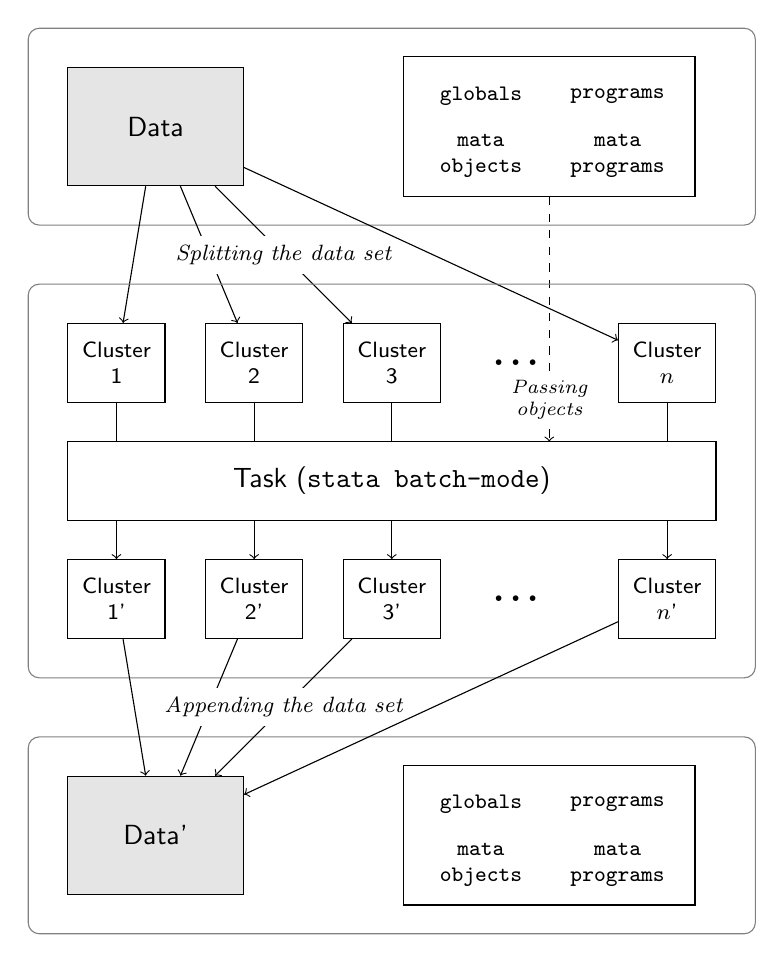
\begin{tikzpicture}[
	every node/.style={node distance=.5cm and .5cm, font=\sffamily}, 
	datablock/.style={rectangle, draw, fill=black!10, text width=2cm, minimum height=1.5cm, text badly centered},
	cluster/.style={rectangle, draw,text width=1cm, text badly centered, minimum height=1cm, font=\footnotesize\sffamily},
	explain/.style={rectangle, text width=5.5cm, align=left, font=\footnotesize\sffamily, node distance=.3, scale=.9}
	] 
	
\node [rectangle, draw=gray, text width=9cm, minimum height=2.5cm, rounded corners] (stata instance0) at (0,0) {};

% Original data
\node [datablock] (data) at (-3,0) {Data};
\matrix [
	draw=black,
	nodes={
		rectangle, text width=1.5cm, minimum height=.75cm, 
		scale=1,
		font=\tt\footnotesize, text badly centered}, column sep=0, row sep=0
	] (others) at (2,0) {
	\node {globals};& \node {programs}; \\
	\node {mata objects}; & \node {mata programs}; \\
};

% Data clusters
\node [cluster] (cluster3) at (0,-3) {Cluster 3};
\node [cluster, left=of cluster3] (cluster2) {Cluster 2};
\node [cluster, left=of cluster2] (cluster1) {Cluster 1};
\node [rectangle, right=of cluster3, text width=1cm, font=\Huge] (threepoints) {...};
\node [cluster, right=of threepoints,text badly centered] (clustern) {Cluster $n$};

% Splitting
\draw[->] (data) -- (cluster1);
\draw[->] (data) -- (cluster2);
\draw[->] (data) -- node [fill=white, font=\footnotesize\it] {Splitting the data set} (cluster3);
\draw[->] (data) -- (clustern);

\draw[->, dashed] (others) -- node [fill=white, font=\scriptsize\it, below=.65cm, text width=1.2cm, minimum height=.7cm,text badly centered] {Passing objects} (2,-4);

% Procesed clusters
\node [cluster] (cluster3p) at (0,-6) {Cluster 3'};
\node [cluster, left=of cluster3p] (cluster2p) {Cluster 2'};
\node [cluster, left=of cluster2p] (cluster1p) {Cluster 1'};
\node [rectangle, right=of cluster3p, text width=1cm, font=\Huge] (threepointsp) {...};
\node [cluster, right=of threepointsp,text badly centered] (clusternp) {Cluster $n$'};

\draw[->] (cluster1) -- (cluster1p);
\draw[->] (cluster2) -- (cluster2p);
\draw[->] (cluster3) -- (cluster3p);
\draw[->] (clustern) -- (clusternp);

% Task
\node [rectangle, draw=gray, text width=9cm, minimum height=5cm, rounded corners] (stata batch) at (0,-4.5) {};
\node [rectangle, fill=white, draw, text width=8cm, text badly centered,minimum height=1cm] (task) at (0,-4.5) {Task (\texttt{stata batch-mode})};

% Result
\node [rectangle, draw=gray, text width=9cm, minimum height=2.5cm, rounded corners] (stata instance1) at (0,-9) {};
\node [datablock] (datap) at (-3,-9) {Data'};
\matrix [
	draw=black,
	nodes={
		rectangle, text width=1.5cm, minimum height=.75cm, 
		scale=1,
		font=\tt\footnotesize, text badly centered}, column sep=0, row sep=0
	] (othersp) at (2,-9) {
	\node {globals};& \node {programs}; \\
	\node {mata objects}; & \node {mata programs}; \\
};

\draw[->] (cluster1p) -- (datap);
\draw[->] (cluster2p) -- (datap);
\draw[->] (cluster3p) -- node [fill=white, font=\footnotesize\it] {Appending the data set} (datap);
\draw[->] (clusternp) -- (datap);

% Text
%\node [explain, right=of stata instance0] {Starting (current) {\tt stata} instance loaded with data plus user defined {\tt globals}, {\tt programs}, {\tt mata objects} and {\tt mata programs}};

%\node [explain, right=of stata batch] {A new {\tt stata} instance (batch-mode) for every data-clusters. Programs, globals and mata objects/programs are passed to them.\\\bigskip The same algorithm (task) is simultaneously applied over the data-clusters.\\\bigskip After every instance stops, the data-clusters are appended into one.};

%\node [explain, right=of stata instance1] {Ending (resulting) {\tt stata} instance loaded with the new data.\\\bigskip User defined {\tt globals}, {\tt programs}, {\tt mata objects} and {\tt mata programs} remind unchanged.};

\end{tikzpicture}
}
\end{figure}
\end{frame}

\begin{frame} % [allowframebreaks=.8]
\frametitle{What is it and how does it work}
\framesubtitle{How does it work?}

\begin{itemize}
\item Method is \textit{split-apply-combine} like MapReduce. Very flexible!\pause{}
\item Straightforward usage when there is observation- or group-level work\pause{}
\item If each iteration needs the entire dataset, then use procedure to split the tasks and load the data separately. Examples\pause{}
\begin{itemize}
\item Table of seeds for each bootstrap resampling\pause{}
\item Table of parameter values for simulations\pause{}
\end{itemize}
\item If the list of tasks is data-dependent then the ``nodata'' alternative mechanism allows for more flexibility.
\end{itemize}

\end{frame}


\begin{frame}
\frametitle{Implementation }
\begin{itemize}
\item Uses shell on Linux/MacOS. On Windows we have a compiled plugging allowing\pause{}
\begin{itemize}
\item Functionality when the parent Stata is in batch-mode\pause{}
\item Seamless user experience by launching the child programs in a hidden desktop (otherwise GUI for each steals focus)\pause{}
\end{itemize}
\item For a computer cluster with a shared filesystem (e.g. NFS) can distribute across nodes. \pause{}
\begin{itemize}
\item New feature so we'd appreciate help from the community to extend to other cluster settings (e.g. \href{https://en.wikipedia.org/wiki/Portable_Batch_System}{PBS})\pause{}
\end{itemize}

\end{itemize}
\end{frame}

%\begin{frame}
%\frametitle{What is it and how does it work}
%{\Large Sounds ``pretty'' but\ldots}\pause{} {\Huge is this for real!?}
%\end{frame}

%\begin{frame}
%\frametitle{What is it and how does it work}
%\framesubtitle{Parallel's backend}
%When the user enters 
%\begin{figure}[fragile]
%\small
%\centering
%{\bf{\tt parallel: gen x2 = x*x}}
%\end{figure} 
%{\tt parallel} takes the command and writes something like this\pause{}
%\bigskip
%\scriptsize
%\scalebox{.9}{
%\def\anchomini{.6\textwidth}
\begin{minipage}[c]{\anchomini}
\begin{semiverbatim}
  cap clear all
  cd ~
1 {\bf{}set seed 34815}
  set memory 16777216b
  cap set maxvar 5000
  cap set matsize 400
2 {\bf{}local pll\_instance 1}
  local pll_id efcql2tspr
  capture \{
  noisily \{
3 {\bf{}use \_\_pllefcql2tsprdataset if \_efcql2tsprcut == 1}
  {\bf{}gen n = \_N}
  \}
  \}
4 {\bf{}save \_\_pllefcql2tsprdta1, replace}
  local result = _rc
  cd ~
5 {\bf{}mata: write\_diagnosis(st\_local("result"),}
  >{\bf{}"\_\_pllefcql2tsprfinito1")}
\end{semiverbatim}
\end{minipage}\pause{}
% SPLIT
\begin{minipage}[c]{\anchomini}
\begin{semiverbatim}
  cap clear all
  cd ~
1 {\bf{}set seed 98327}
  set memory 16777216b
  cap set maxvar 5000
  cap set matsize 400
2 {\bf{}local pll\_instance 2}
  local pll_id efcql2tspr
  capture \{
  noisily \{
3 {\bf{}use \_\_pllefcql2tsprdataset if \_efcql2tsprcut == 2}
  {\bf{}gen n = \_N}
  \}
  \}
4 {\bf{}save \_\_pllefcql2tsprdta2, replace}
  local result = _rc
  cd ~
5 {\bf{}mata: write\_diagnosis(st\_local("result"),}
  >{\bf{}"\_\_pllefcql2tsprfinito2")}
\end{semiverbatim}
\end{minipage}

%}
%\end{frame}


%\begin{frame}
%\frametitle{What is it and how does it work}
%{\Large Ok, it works but\ldots}\pause{} 
%
%{\Huge it must be really hard to use!}
%\end{frame}

\section{Benchmarks}
\frame{\tableofcontents[currentsection]}


%Old timings so disable for now
%\begin{frame}[b,fragile]
%\frametitle{Benchmarks}
%\framesubtitle{Simple example: Serial replace}
%\begin{minipage}[c]{1\textwidth}
%\begin{minipage}[c]{.35\textwidth}
%Serial fashion
%\begin{semiverbatim}\scriptsize
%do mydofile.do
%\end{semiverbatim}
%Parallel fashion
%\begin{semiverbatim}\scriptsize
%parallel do mydofile.do
%\end{semiverbatim}
%\end{minipage}
%%SPLIT
%\fbox{
%\begin{minipage}[c]{.6\textwidth}\scriptsize
%\begin{figure}
%\caption{mydofile.do}
%\begin{semiverbatim}
%local size = \_N
%forval i=1/`size' \{
%\hspace{1cm}qui replace x = ///
%\hspace{1.5cm}1/sqrt(2*`c(pi)')*exp(-(x\^{}2/2)) in `i'
%\}
%\end{semiverbatim}
%\end{figure}
%\end{minipage}}
%\end{minipage}
%\begin{table}[!h]
%\centering
%\caption{Serial replacing using a loop on a Linux Server (16 clusters)}
%\scalebox{.9}{
%\begin{tabular}{l*{3}{c}}\toprule
%& 100,000 &         1,000,000 &       10,000,000 \\ \midrule
%CPU &     1.43 &     16.94 &    144.68 \\
%Total &     0.34 &      3.20 &     12.49 \\
%\hspace{2mm} Setup &     0.00 &      0.00 &      0.00 \\
%\hspace{2mm} Compute &     0.32 &      3.07 &     11.54 \\
%\hspace{2mm} Finish &     0.02 &      0.12 &      0.95 \\
%\midrule Ratio (compute) &     4.50 &      5.51 &     12.53 \\
%Ratio (total) &     4.22 (26\%) &      5.30 (30\%) &     11.58 (72\%) \\
%\bottomrule
%\multicolumn{4}{l}{\footnotesize Tested on a \unix1 machine}
%\end{tabular}}
%\end{table}
%\end{frame}

%Old timings so disable for now
%\begin{frame}[b,fragile]
%\frametitle{Benchmarks}
%\framesubtitle{Monte Carlo simulation (Windows Machine)}
%\begin{minipage}[c]{1\textwidth}
%\begin{minipage}[c]{.45\textwidth}
%\bigskip
%Serial fashion
%\begin{semiverbatim}\scriptsize
%do myexperiment.do
%\end{semiverbatim}
%Parallel fashion
%\begin{semiverbatim}\scriptsize
%parallel do myexperiment.do, nodata
%\end{semiverbatim}
%\end{minipage}
%%SPLIT
%\fbox{
%\scalebox{.4}{
%\begin{minipage}[c]{1\textwidth}\scriptsize
%\begin{figure}
%{\Huge \caption{myexperiment.do}}
%\begin{semiverbatim}
%local num\_of\_intervals = 50
%if length("`pll\_id'") == 0 \{
%\hspace{.5cm}local start = 1
%\hspace{.5cm}local end = `num\_of\_intervals'
%\}
%else \{
%\hspace{.5cm}local ntot = floor(`num\_of\_intervals'/\$PLL\_CLUSTERS)
%\hspace{.5cm}local start = (`pll\_instance' - 1)*`ntot' + 1
%\hspace{.5cm}local end = (`pll\_instance')*`ntot'
%\hspace{.5cm}if `pll\_instance' == \$PLL\_CLUSTERS local end = 10
%\}
%local reps 10000
%forval i=`start'/`end' \{
%\hspace{.5cm}qui use census2, clear
%\hspace{.5cm}gen true\_y = age
%\hspace{.5cm}gen z\_factor = region
%\hspace{.5cm}sum z\_factor, meanonly
%\hspace{.5cm}scalar zmu = r(mean)
%\hspace{.5cm}qui \{
%\hspace{.5cm}\hspace{.5cm}gen y1 = .
%\hspace{.5cm}\hspace{.5cm}gen y2 = .
%\hspace{.5cm}\hspace{.5cm}local c = `i'
%\hspace{.5cm}\hspace{.5cm}set seed `c'
%\hspace{.5cm}\hspace{.5cm}simulate c=r(c) mu1=r(mu1) se\_mu1 = r(se\_mu1) ///
%\hspace{.5cm}\hspace{.5cm}\hspace{.5cm}\hspace{.5cm}mu2=r(mu2) se\_mu2 = r(se\_mu2), /// 
%\hspace{.5cm}\hspace{.5cm}\hspace{.5cm}\hspace{.5cm}saving(cc`i', replace) nodots reps(`reps'): ///
%\hspace{.5cm}\hspace{.5cm}\hspace{.5cm}\hspace{.5cm}mcsimul1, c(`c')
%\hspace{.5cm}\}
%\}
%\end{semiverbatim}
%\end{figure}
%\end{minipage}}}
%\end{minipage}
%\begin{table}[!h]
%\centering
%\caption{Monte Carlo Experiment on a Windows Machine (4 clusters)}
%\scalebox{.85}{
%\begin{tabular}{l*{2}{c}}\toprule
%& 2 &               4 \\ \midrule
%CPU &   111.49 &    114.13 \\
%Total &    58.02 &     37.48 \\
%\hspace{2mm} Setup &     0.00 &      0.00 \\
%\hspace{2mm} Compute &    58.02 &     37.48 \\
%\hspace{2mm} Finish &     0.00 &      0.00 \\
%\midrule Ratio (compute) &     1.92 &      3.04 \\
%Ratio (total) &     1.92 (96\%)&      3.04 (76\%)\\
%\bottomrule
%\multicolumn{3}{l}{\footnotesize Tested on a \windows1 machine}
%\end{tabular}}
%\end{table}
%\end{frame}

%Old timings so disable for now
%\begin{frame}[b]
%\frametitle{Benchmarks}
%\framesubtitle{Monte Carlo simulation (Unix Machine) and Reshaping Administrative Data}
%\bigskip
%Serial fashion
%\begin{semiverbatim}
%\scriptsize
%do myexperiment.do
%\end{semiverbatim}
%Parallel fashion
%\begin{semiverbatim}
%\scriptsize
%parallel do myexperiment.do, nodata
%\end{semiverbatim}
%\begin{table}[!h]
%\centering
%\caption{Monte Carlo Experiment on a Linux Server (16 clusters)}
%\scalebox{.85}{
%\begin{tabular}{l*{4}{c}}\toprule
%& 2 &               4 &               8 &              16 \\ \midrule
%CPU &   164.79 &    164.04 &    162.84 &    163.89 \\
%Total &    69.85 &     34.28 &     19.00 &     10.78 \\
%\hspace{2mm} Setup &     0.00 &      0.00 &      0.00 &      0.00 \\
%\hspace{2mm} Compute &    69.85 &     34.28 &     19.00 &     10.78 \\
%\hspace{2mm} Finish &     0.00 &      0.00 &      0.00 &      0.00 \\
%\midrule Ratio (compute) &     2.36 &      4.78 &      8.57 &     15.21 \\
%Ratio (total) &     2.36 (118\%) &      4.78 (120\%)&      8.57 (107\%) &     15.21 (95\%) \\
%\bottomrule
%\multicolumn{4}{l}{\footnotesize Tested on a \unix1 machine}
%\end{tabular}}
%\end{table}
%\end{frame}

%Old timings so disable for now
%\begin{frame}[b]
%\frametitle{Benchmarks}
%\framesubtitle{Reshaping Administrative Data}
%\bigskip
%Serial fashion
%\begin{semiverbatim}
%\scriptsize
%reshape wide tipsolic rutemp opta derecho ngiros, ///
%\hspace{1cm}i(id) j(time)
%\end{semiverbatim}
%Parallel fashion
%\begin{semiverbatim}
%\scriptsize
%parallel, by(id) :reshape wide tipsolic rutemp opta derecho ngiros, ///
%\hspace{1cm}i(id) j(time)
%\end{semiverbatim}
%\begin{table}[!h]
%\centering
%\caption{Reshaping wide a large database on a Linux Server (8 clusters)}
%\scalebox{.8}{
%\begin{tabular}{l*{3}{c}}\toprule
%& 100,000 &         1,000,000 &         5,000,000 \\ \midrule
%CPU &     5.51 &     72.70 &    392.97 \\
%Total &     2.33 &     17.46 &     86.44 \\
%\hspace{2mm} Setup &     0.00 &      0.00 &      0.00 \\
%\hspace{2mm} Compute &     1.83 &     12.42 &     57.93 \\
%\hspace{2mm} Finish &     0.50 &      5.04 &     28.51 \\
%\midrule Ratio (compute) &     3.01 &      5.85 &      6.78 \\
%Ratio (total) &     2.37 (29\%)&      4.16 (52\%)&      4.55 (57\%)\\
%\bottomrule
%\multicolumn{4}{l}{\footnotesize Tested on a \unix1 machine}
%\end{tabular}}
%\end{table}
%\end{frame}


\begin{frame}[t]
\frametitle{Benchmarks}
\framesubtitle{Bootstrap with \tt{parallel bs}}
\begin{semiverbatim}
	\scriptsize
sysuse auto, clear
expand 10


// Serial fashion

bs, rep(\$size) nodots: regress mpg weight gear foreign


// Parallel fashion
parallel setclusters \$number\_of\_clusters

parallel bs, rep(\$size) nodots: regress mpg weight gear foreign
\end{semiverbatim}


\begin{table}[!h]
\centering\begin{tabular}{l*{3}{c}}
	\toprule
	Problem size & Serial & 2 Clusters & 4 Clusters\\\midrule
	1,000 &   2.93s &   1.62s &   1.09s \\    
	&  $\times$2.69 &  $\times$1.48 &  $\times$1.00 \\ \\
	2,000 &   5.80s &   3.13s &   2.03s \\    
	&  $\times$2.85 &  $\times$1.54 &  $\times$1.00 \\ \\
	4,000 &  11.59s &   6.27s &   3.86s \\    
	&  $\times$3.01 &  $\times$1.62 &  $\times$1.00 \\
	\bottomrule
\end{tabular}
\caption{Absolute and relative computing times for each run of a basic bootstrap problem. For each given problem size, the first row shows the time in seconds, and the second row shows the relative time each method took to complete the task relative to using parallel with four clusters. Each cell represents a 1,000 runs.}
	\end{table}
	
\end{frame}

\begin{frame}[t]
	\frametitle{Benchmarks}
	\framesubtitle{Simulations with \tt{parallel sim}}
	\begin{semiverbatim}
		\scriptsize
prog def mysim, rclass

\hspace{.5cm}// Data generating process

\hspace{.5cm}drop \_all

\hspace{.5cm}set obs 1000 

\hspace{.5cm}gen eps = rnormal()

\hspace{.5cm}gen X   = rnormal()

\hspace{.5cm}gen Y   = X*2 + eps 


\hspace{.5cm}// Estimation

\hspace{.5cm}reg Y X 

\hspace{.5cm}mat def ans = e(b)

\hspace{.5cm}return scalar beta = ans[1,1]

end


// Serial fashion

simulate beta=r(beta), reps(\$size) nodots: mysim


// Parallel fashion

parallel setclusters \$number\_of\_clusters

parallel sim, reps(\$size) expr(beta=r(beta)) nodots: mysim
	\end{semiverbatim}
	
\end{frame}

\begin{frame}[t]
	\frametitle{Benchmarks}
	\framesubtitle{Simulations with \tt{parallel sim} (cont.)}
	
	\begin{table}[!h]
\centering\begin{tabular}{l*{3}{c}}
	\toprule
	Problem size & Serial & 2 Clusters & 4 Clusters\\\midrule
	1000 &   2.19s &   1.18s &   0.73s \\    
	&  $\times$3.01 &  $\times$1.62 &  $\times$1.00 \\ \\
	2000 &   4.36s &   2.29s &   1.33s \\    
	&  $\times$3.29 &  $\times$1.73 &  $\times$1.00 \\ \\
	4000 &   8.69s &   4.53s &   2.55s \\    
	&  $\times$3.40 &  $\times$1.77 &  $\times$1.00 \\
	\bottomrule
\end{tabular}
		\caption{Absolute and relative computing times for each run of a simple Monte Carlo exercise. For each given problem size, the first row shows the time in seconds, and the second row shows the relative time each method took to complete the task relative to using parallel with four clusters. Each cell represents a 1,000 runs.}
	\end{table}
	
Code for replicating this is available at \url{https://github.com/gvegayon/parallel}
	
\end{frame}

\section{Syntax and Usage}

\frame{\tableofcontents[currentsection]}

\begin{frame}
\frametitle{Syntax and Usage}

Setup

\begin{semiverbatim}
\footnotesize
{\bf parallel setclusters} \textit{\#}|default  [, \uline{f}orce \uline{h}ostnames(namelist)] 
%Infrequent options: statapath(), includefile(), ssh()
\end{semiverbatim}\pause{}

Main command types

\begin{semiverbatim}
\footnotesize
{\bf parallel} [, by(\textit{\color{blue} varlist}) \uline{p}rograms(\textit{\color{blue} namelist}) \uline{m}ata \uline{s}eeds(\textit{\color{blue} string}) \uline{r}andtype(\textit{\color{blue} random.org$|$datetime})

\hspace{1cm} \uline{nod}ata]:  \textit{stata\_cmd}
%Infrequent options: force, setparallelid(). processors(), keep, keeplast, noglobal, timeout(), outputopts(), deterministicoutput
\end{semiverbatim}\pause{}

\begin{semiverbatim}
\footnotesize
{\bf parallel do} \textit{\color{blue} filename} [, by(\textit{\color{blue} varlist}) \uline{p}rograms(\textit{\color{blue} namelist}) \uline{m}ata \uline{s}eeds(\textit{\color{blue} string})

\hspace{1cm}  \uline{r}andtype(\textit{\color{blue} random.org$|$datetime}) \uline{nod}ata]
%Infrequent options: force, setparallelid(). processors(), keep, keeplast, noglobal, timeout(), outputopts(), deterministicoutput
\end{semiverbatim}\pause{}

Helper commands

\begin{semiverbatim}
	\footnotesize
	{\bf parallel bs} [, \uline{exp}ression(\textit{\color{blue} exp\_list}) \uline{p}rograms(\textit{\color{blue} namelist}) \uline{m}ata \uline{s}eeds(\textit{\color{blue} string}) 
	
	\hspace{1cm} \uline{r}andtype(\textit{\color{blue} random.org$|$datetime}) \textit{bs\_options}]:  \textit{stata\_cmd}
%Infrequent options: processors(), keep, keeplast, noglobal, timeout(), outputopts(), deterministicoutput
\end{semiverbatim}\pause{}

\begin{semiverbatim}
	\footnotesize
	{\bf parallel sim} [, \uline{exp}ression(\textit{\color{blue} exp\_list}) \uline{p}rograms(\textit{\color{blue} namelist}) \uline{m}ata \uline{s}eeds(\textit{\color{blue} string})
	
	\hspace{1cm} \uline{r}andtype(\textit{\color{blue} random.org$|$datetime}) \textit{sim\_options})]:  \textit{stata\_cmd}
%Infrequent options: processors(), keep, keeplast, noglobal, timeout(), outputopts(), deterministicoutput
\end{semiverbatim}\pause{}

\begin{semiverbatim}
	\footnotesize
	{\bf parallel append} [\textit{files}], do(\textit{\color{blue} command|dofile}) [in(\textit{\color{blue} in}) if(\textit{\color{blue} if}) \uline{exp}ression(\textit{\color{blue} expand\_exp})
	
	\hspace{1cm} \uline{p}rograms(\textit{\color{blue} namelist}) \uline{m}ata \uline{s}eeds(\textit{\color{blue} string}) \uline{r}andtype(\textit{\color{blue} random.org$|$datetime})]
%Infrequent options: processors(), keep, keeplast, noglobal, timeout(), outputopts(), deterministicoutput
\end{semiverbatim}\pause{}

Additional Utilities
\begin{semiverbatim}
	\footnotesize
	{\bf parallel version}/{\bf clean}/{\bf printlog}/{\bf viewlog}/{\bf numprocessors}
%Infrequent options: . event, all, force. event. event.
\end{semiverbatim}

\end{frame}


\begin{frame}
\frametitle{Syntax and Usage}
\framesubtitle{Recommendations on its usage}

\begin{columns}
\begin{column}{.5\textwidth}
{\color{gray}
{\tt parallel suits \ldots}
\rule{\linewidth}{4pt}}
\begin{itemize}
\item Monte-Carlo simulation.\pause{}
\item Extensive nested control flow (loops, while, ifs, etc.).\pause{}
\item Bootstrapping/Jackknife.\pause{}
\item Multiple MCMC chains to test for convergence (Gelman-Rubin test).\pause{}
\item Simulations in general.\pause{}
\end{itemize}
\end{column}%
\hfill%
\begin{column}{.5\textwidth}
{\color{gray}
{\tt parallel doesn't suit \ldots}
\rule{\linewidth}{4pt}}
\begin{itemize}
\item (already) fast commands.\pause{}
\item Regressions, ARIMA, etc.\pause{}
\item Linear Algebra.\pause{}
\item Whatever StataMP does better.\pause{}
\item (Currently) Tasks that already take up all of RAM.
\end{itemize}
\end{column}%
\end{columns}
\end{frame}


\begin{frame}
\frametitle{Use in other Stata modules}

\begin{itemize}
\item \href{https://ideas.repec.org/c/boc/bocode/s458086.html}{EVENTSTUDY2}: Perform event studies with complex test statistics 
\item \href{https://ideas.repec.org/c/boc/bocode/s457822.html}{MIPARALLEL}: Perform parallel estimation for multiple imputed datasets 
\item \href{https://github.com/bquistorff/synth_runner}{Synth\_Runner}: Performs multiple Synthetic Control estimations for permutation testing 

\end{itemize}

\end{frame}

\section{Concluding Remarks}

\begin{frame}
\frametitle{Concluding Remarks}

\begin{itemize}
\item Brings parallel computing to many more commands than StataMP \pause{}
\item Its major strengths/advantages are in simulation models and non-vectorized operations such as control-flow statements.\pause{}
\item Depending on the proportion of the algorithm that can be parallelized, it is possible to reach near to linear scale speedups.\pause{}
\item We welcome other user commands optionally including {\tt parallel} for speedup. \pause{}
%\item Caveat: Has not been tested yet on Stata 15.\pause{}
\item Contribute, find help, and report bugs at \url{http://github.com/gvegayon/parallel}\pause{}

\end{itemize}

\end{frame}

\title{Thank you very much!}

\frame{\maketitle
}

\end{document}
